\chapter{Vergleich AOT vs. JIT}

\section{Programmausführung in der VM} \label{jit_vm}
Durch die Dynamik einer Programmiersprache, zur Schaffung einer Plattformunabhängigkeit oder aus Sicherheitsgründen werden Programme heutzutage oftmals nicht mehr direkt vom Betriebssystem ausgeführt, sondern laufen in einer \ac{VM}, wie dies bereits bei Smaltalk-80 der Fall war. Dies verzögert jedoch die Ausführungszeit der Interpretation der Befehle. \\
Durch die Anwendung von \ac{JIT} wird hier versucht Performance zu gewinnen und somit diesen Nachteil auszugleichen. Folgend sollen die beiden \ac{VM}'s 'HotSpot' und 'Graal' aus dem Kontext der Sprache Java näher vorgestellt werden. 
\subsection{HotSpot}
Java übersetzt den Code der Hochsprache generell zuerst in Bytecode, der in der \ac{VM} ausgeführt werden kann. Diese \ac{VM} wird speziell für das korrespondierende \ac{OS} bereitgestellt und kann auf dieser Plattform den erzeugten Bytecode korrekt ausführen. 'HotSpot' von Oracle ist eine dieser \ac{VM}'s für die Sprache Java. \\
\\
\begin{figure}[ht]
    \begin{center}
        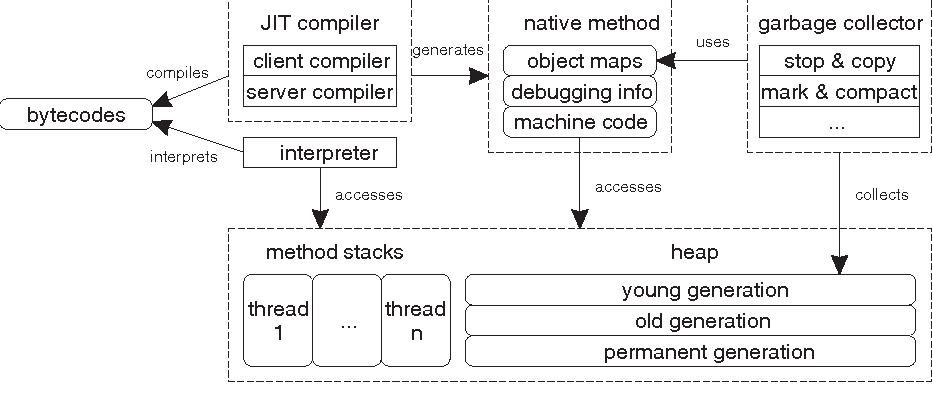
\includegraphics[width=0.9\textwidth]{assets/img/3-Figure1-1.png}
        \caption{Architektur 'HotSpot', \cite[Quelle: Kotzmann Wimmer 2008]{KotzmannWimmer2008}}
        \label{arch_hotspot}
    \end{center}
\end{figure}
Wie in \autoref{arch_hotspot} zu sehen, beginnt die Ausführung in der 'HotSpot'-\ac{VM} beim Interpreter. Hier wird der Bytecode schrittweise ausgeführt anhand von Templates ausgeführt. Nur die heuristisch am meisten frequentierten Codeblöcke werden durch den \ac{JIT}-Compiler kompiliert.\\
Wird während der Ausführung eine besonders aufwändige Schleife entdeckt, so wird diese ebenfalls kompiliert und die Ausführung dafür gestoppt. Die Schwierigkeit besteht hierbei darin, dass die Ausführung zwischen Interpreter und dem kompilierten Code synchronisiert werden muss. Dafür wird ein neuer Stackframe erstellt und initialisiert. Die Ausführung der Methode geht im nativen Code weiter. Dieses Verfahren nennt man \ac{OSR}.\\
'HotSpot' enthält zwei verschiedene Compiler, die für Server- und Clientsysteme gedacht sind. Bei Serversystemen wird sehr großer Wert auf eine sehr gute Optimierung gelegt, dafür jedoch eine längere Kompilierungszeit in Kauf genommen. Für dauerhaft laufende Serveranwendungen geht man davon aus, dass bereits während der Anlaufphase der Software der \ac{JIT}-Compiler alle wichtigen Methoden und Blöcke kompiliert und optimiert. Die längere Zeit ist hierfür nicht relevant, da die einmal kompilierten Sequenzen danach während der ganzen Laufzeit der Software zu Verfügung stehen.\\
Der Compiler für die Clientsysteme zielt auf Programme mit \ac{GUI} ab. Hier wird der Fokus auf die Antwortzeit der Oberfläche und damit den Punkt \ac{UX} gelegt. Dazu ist der \ac{JIT}-Compiler auf eine schnelle Kompilierung statt Performance ausgelegt.\\
Reservierter Speicher wird in drei Bereichen verwaltet. Neu kompilierte Methoden werden zuerst im Bereich der 'Young Generation' abgelegt. Füllt sich dieser Bereich, wird eine 'stop-and-copy' \ac{GC} initialisiert. Diese prüft, ob ein Objekt noch in Benutzung ist und löscht alle übrigen, um Speicher wieder freizugeben. Übersteht eine Methode mehrere Runden, wird sie in den Bereich der 'Old Generation' übernommen. Der Dritte Bereich wird als 'Permanent Generation' bezeichnet und enthält interne Datenstrukturen. Dieses Schema ist in \autoref{arch_hotspot} dargestellt, \cite[vgl. Kotzmann und Wimmer 2008, S.3f]{KotzmannWimmer2008}.\\

\subsection{Graal}

% TODO Experiment selbst ausführen oder aus Paper klauen?
% \section{}